% Schema "Hypothesis testing" (replica di img/great_pic.png)
% Compile from class3/: pdflatex great_pic_crust.tex
%   then: pdftocairo -png -transp -singlefile -scale-to-x 2362 -scale-to-y -1 great_pic_crust.pdf img/great_pic_crust
\documentclass[tikz,border=0pt]{standalone}
\usepackage[T1]{fontenc}
\usepackage{lmodern}
\usepackage{amsmath}
\usetikzlibrary{arrows.meta,shapes.geometric}

\definecolor{titleblue}{RGB}{58,59,145}
\definecolor{arrowgray}{RGB}{78,78,78}
\definecolor{outline}{RGB}{45,45,58}
\definecolor{rock}{RGB}{108,112,128}
\definecolor{rockdark}{RGB}{62,66,80}
\definecolor{handle}{RGB}{222,160,82}
\definecolor{grip}{RGB}{125,80,40}
\definecolor{steel}{RGB}{160,168,186}
\definecolor{burst}{RGB}{255,214,60}

% Gruppi e testi (modificare qui se necessario)
\newcommand{\gA}{\text{thin}}
\newcommand{\gB}{\text{thick}}
\newcommand{\nA}{\text{tn}}
\newcommand{\nB}{\text{tc}}
\newcommand{\ideatext}{Magmas erupting through thick crust\\are more differentiated}
\newcommand{\datatitle}{Data: SiO$_2$ content}

\begin{document}
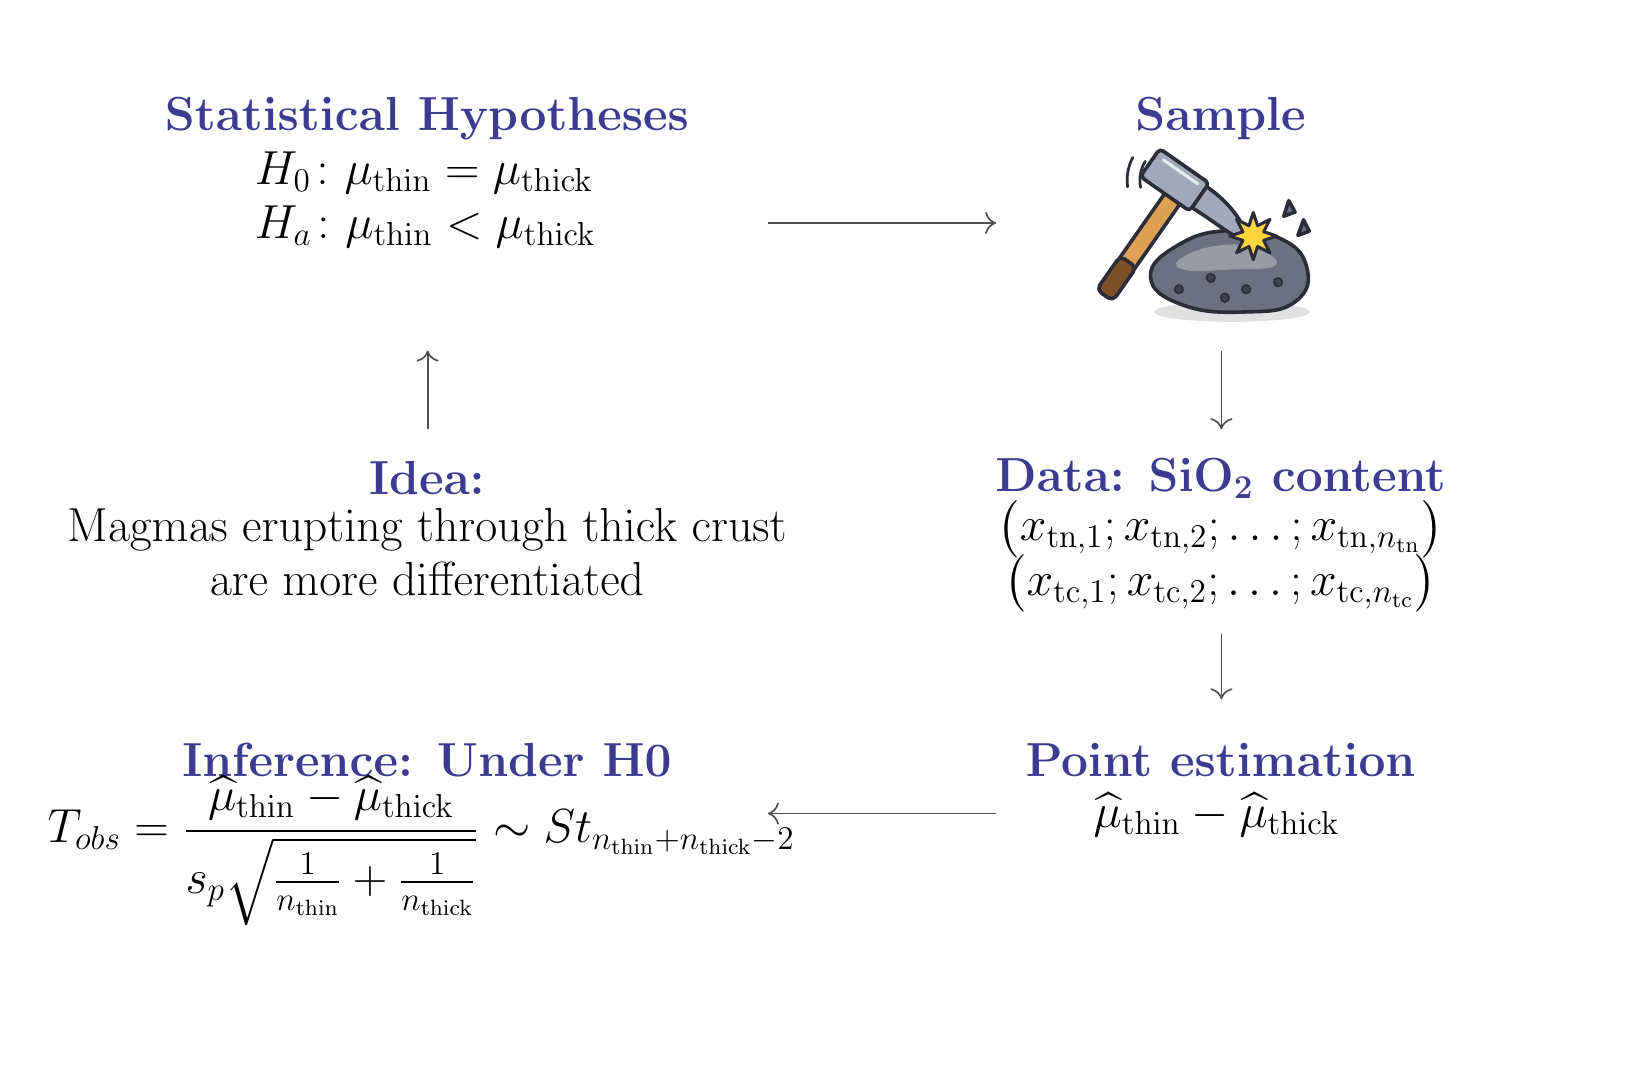
\begin{tikzpicture}[x=1cm,y=1cm,
    every node/.style={inner sep=0pt, outer sep=0pt},
    title/.style={text=titleblue, font=\fontsize{18.3}{22}\selectfont\bfseries\boldmath},
    body/.style={font=\fontsize{17}{19.5}\selectfont, align=center},
    flow/.style={draw=arrowgray, line width=0.6pt, -{To[length=4pt,width=8pt]}}]

  % Tela con le stesse proporzioni dell'immagine originale
  \path[use as bounding box] (0,0) rectangle (20,-12.87);

  % --- Statistical Hypotheses -------------------------------------------
  \node[title] at (5.07,-1.15) {Statistical Hypotheses};
  \node[body, align=left, anchor=north] at (5.05,-1.58)
    {$H_0\colon \mu_{\gA} = \mu_{\gB}$\\
     $H_a\colon \mu_{\gA} < \mu_{\gB}$};

  % --- Sample -------------------------------------------------------------
  \node[title] at (15.15,-1.15) {Sample};
  % cartoon rock hammer striking a rock sample (no frame)
  \begin{scope}[shift={(15.16,-2.62)}, scale=0.9, line cap=round, line join=round,
                ol/.style={draw=outline, line width=1.3pt}]
    % ground shadow
    \fill[black, opacity=0.12] (0.15,-1.1) ellipse (1.1 and 0.14);
    % rock
    \filldraw[fill=rock, ol] plot[smooth cycle, tension=0.8] coordinates
      {(-0.6,-0.15) (0.1,0.05) (0.8,-0.05) (1.2,-0.45) (1.05,-0.95) (0.35,-1.1) (-0.55,-1.0) (-1.0,-0.6)};
    \fill[white, opacity=0.3] plot[smooth cycle, tension=0.8] coordinates
      {(-0.5,-0.3) (0.1,-0.15) (0.6,-0.25) (0.75,-0.45) (0.2,-0.5) (-0.55,-0.5)};
    \foreach \c in {(-0.15,-0.62),(0.35,-0.78),(0.8,-0.68),(0.05,-0.9),(-0.6,-0.78)}
      \filldraw[fill=rockdark, draw=outline, line width=0.6pt] \c circle (0.06);
    % hammer (upper left)
    \begin{scope}[shift={(-0.9,0.2)}, rotate=-35]
      \filldraw[fill=handle, ol, rounded corners=2pt] (-0.13,-1.3) rectangle (0.13,0.5);
      \filldraw[fill=grip, ol, rounded corners=2pt] (-0.14,-1.3) rectangle (0.14,-0.72);
      \filldraw[fill=steel, ol, rounded corners=1.5pt] (-0.55,0.36) rectangle (0.3,0.84);
      \filldraw[fill=steel, ol] (0.3,0.42) .. controls (0.8,0.44) and (1.05,0.4) .. (1.25,0.5)
                                .. controls (1.05,0.62) and (0.8,0.78) .. (0.3,0.78) -- cycle;
      \draw[white, line width=1.1pt, opacity=0.75] (-0.42,0.74) -- (0.18,0.74);
    \end{scope}
    % swing lines behind the head
    \draw[outline, line width=1pt] ([shift={(-0.65,0.76)}] 148:0.5) arc (148:192:0.5);
    \draw[outline, line width=1pt] ([shift={(-0.65,0.76)}] 152:0.68) arc (152:188:0.68);
    % impact burst + chips
    \node[star, star points=8, star point ratio=2.1, fill=burst, draw=outline, line width=1.1pt,
          minimum size=0.6cm, inner sep=0pt] at (0.45,-0.03) {};
    \filldraw[fill=rock, ol] (0.88,0.25) -- (1.04,0.31) -- (0.95,0.47) -- cycle;
    \filldraw[fill=rock, ol] (1.08,-0.02) -- (1.24,0.04) -- (1.16,0.2) -- cycle;
  \end{scope}

  % --- Data ---------------------------------------------------------------
  \node[title] at (15.15,-5.72) {\datatitle};
  \node[body, anchor=north] at (15.15,-6.00)
    {$\bigl(x_{\nA,1}; x_{\nA,2}; \ldots; x_{\nA,n_{\nA}}\bigr)$\\[-2pt]
     $\bigl(x_{\nB,1}; x_{\nB,2}; \ldots; x_{\nB,n_{\nB}}\bigr)$};

  % --- Point estimation ---------------------------------------------------
  \node[title] at (15.15,-9.3) {Point estimation};
  \node[body] at (15.1,-10.0)
    {$\widehat{\mu}_{\gA} - \widehat{\mu}_{\gB}$};

  % --- Inference ----------------------------------------------------------
  \node[title] at (5.07,-9.3) {Inference: Under H0};
  \node[body] at (5.0,-10.45)
    {$T_{obs} = \dfrac{\widehat{\mu}_{\gA} - \widehat{\mu}_{\gB}}
                      {s_p\sqrt{\frac{1}{n_{\gA}} + \frac{1}{n_{\gB}}}}
       \sim St_{n_{\gA} + n_{\gB} - 2}$};

  % --- Idea ---------------------------------------------------------------
  \node[title] at (5.07,-5.72) {Idea:};
  \node[body, anchor=north] at (5.07,-6.10) {\ideatext};

  % --- Frecce -------------------------------------------------------------
  \draw[flow] (9.40,-2.48)  -- (12.30,-2.48);
  \draw[flow] (15.16,-4.10) -- (15.16,-5.10);
  \draw[flow] (15.16,-7.70) -- (15.16,-8.53);
  \draw[flow] (12.30,-9.98) -- (9.40,-9.98);
  \draw[flow] (5.08,-5.10)  -- (5.08,-4.10);
\end{tikzpicture}
\end{document}
